\documentclass[conference]{IEEEtran}
\IEEEoverridecommandlockouts
% The preceding line is only needed to identify funding in the first footnote. If that is unneeded, please comment it out.
\usepackage{cite}
\usepackage{amsmath,amssymb,amsfonts}
\usepackage{algorithmic}
\usepackage{graphicx}
\usepackage{textcomp}
\usepackage{xcolor}
\usepackage{dblfloatfix}
\usepackage[colorlinks=true, linkcolor=blue, urlcolor=blue, citecolor=green]{hyperref}
\usepackage{minted}
\usepackage{microtype}
%\usepackage{parskip}

\def\BibTeX{{\rm B\kern-.05em{\sc i\kern-.025em b}\kern-.08em
    T\kern-.1667em\lower.7ex\hbox{E}\kern-.125emX}}
\begin{document}

\let\subsectionautorefname\sectionautorefname
\let\subsubsectionautorefname\sectionautorefname
\title{Collaborative Learning\\ \large Una soluzione di reinforcement learning\\ applicata a un nodo router di messaggi\\
{\footnotesize Progetto Machine Learning}
}
\author{\IEEEauthorblockN{Matteo Conti}
\IEEEauthorblockA{\textit{0323728}} \\
\and
\IEEEauthorblockN{Daniele La Prova}
\IEEEauthorblockA{\textit{0320429}} \\
\and
\IEEEauthorblockN{Luca Falasca}
\IEEEauthorblockA{\textit{0334722}} \\
}

\newcommand{\code}[1]{\texttt{#1}}

\maketitle

\begin{abstract}
%TODO:
\end{abstract}

\section{Introduzione}
%TODO:

\subsection{Contesto}
%TODO:

\subsection{Obiettivi}
%TODO:

\section{Metodologia}
%TODO:

\subsection{Modello}
%TODO:

\subsection{Agente}
%TODO:

\subsubsection{AgentFaçade}
L'Agent Façade rappresenta un'interfaccia che espone i metodi necessari per l'interazione con l'agente. Questa soluzione consente di nascondere tutte le interazioni tra i sottosistemi e l'agente, offrendo un'interfaccia unificata per la comunicazione con l'agente stesso. Nella nostra implementazione, non è l'agente a restituire direttamente l'azione da intraprendere; piuttosto, è il simulatore (o, in uno scenario reale, il nodo) che richiede, dato un determinato stato, quale azione intraprendere in quel momento. Ciò implica che il simulatore scandisce il tempo. In questo modo, l'agente non è consapevole del tempo trascorso e può facilmente adattarsi a uno scenario reale.
\subsubsection{AgentFaçade - Configurazione} 
Per utilizzare l'AgentFaçade è necessario configurare l'agente. La configurazione può essere fatta tramite un file in cui è possibile specificare varie caratteristiche dell'agente in modo da poterlo adattare a diversi scenari. La documentazione per la configurazione è disponibile \href{https://github.com/retarded-reward/collaborative-learning/wiki/Agent-Configuration}{qui}. Un'altro parametro di configurazione da specificare all'AgentFaçade è il numero di code presenti nel nodo. Questo parametro è necessario per l'agente in modo da poter generare azioni valide.
\subsubsection{AgentFaçade - Interazione}
Il metodo principale per interagire con l'Agent Façade è \code{get\_action}, che restituisce l'azione da intraprendere in base allo stato attuale. Questo metodo prende in input lo stato attuale e la reward associata all'azione precedente, e restituisce l'azione da intraprendere. All'interno di questo metodo, l'Agent Façade addestra l'agente con l'esperienza passata e interroga l'agente per ottenere l'azione da intraprendere utilizzando l'albero delle Decisions  (vedi \autoref{subsec:Decisions}). L'addestramento non avviene ad ogni chiamata, ma secondo un intervallo di step configurabile. Questo intervallo è necessario per evitare che l'agente si adatti troppo velocemente a uno scenario specifico e non sia in grado di generalizzare, oltre a migliorare le prestazioni computazionali.

\subsubsection{AgentFactory}
L'Agent Factory è una classe che configura e crea diversi agenti disponibili nella libreria. Nel nostro caso, abbiamo utilizzato il DQN (Deep Q Network) e un RandomAgent come benchmark. Inoltre, è stato implementato un decoratore per gli agenti per integrarli dinamicamente con i replay buffer forniti dalla libreria. Utilizzando il metodo \code{create\_agent}, è possibile creare un'istanza di un agente specificando il tipo di agente e i parametri necessari per la configurazione. Questa operazione viene eseguita all'interno dell'AgentFaçade.

\subsubsection{Decisions}
\label{subsec:Decisions}
Lo spazio di decisioni in cui un agente può trovarsi ad operare può estendersi
attraverso
diverse dimensioni, ognuna delle quali rappresenta un parametro che costituisce
tale azione. Ad esempio, nel caso del problema in esame un'azione dell'agente è
rappresentabile da un vettore a tre dimensioni così codificato:
\begin{itemize}
\item Azione[0] = invia o non fare nulla;
\item Azione[1] = preleva pacchetto da coda i, con $i \in [0, \code{num\_queues} - 1]$;
\item Azione[2] = seleziona power source j, $j \in [0, \code{num\_power\_sources} - 1]$.
\end{itemize}
Si noti che non tutte le combinazioni di valori di questi parametri
rappresentino dei punti legali all'interno dello spazio delle azioni.
Ad esempio, se la prima componente è pari a 0 (non fare nulla), allora i valori delle
altre componenti devono essere don't care.

Una soluzione può essere ricorrere a un'enumerazione, ovvero si "schiaccia"
lo spazio delle azioni lungo un'unica dimensione i cui valori sono rappresentati 
dalle sole combinazioni che rappresentano azioni legali. È una soluzione semplice e
immediata, tuttavia comporta alcuni problemi:
\begin{itemize}
    \item la dimensione dello spazio delle azioni aumenta molto velocemente rispetto
    all'aumentare delle opzioni disponibili. Nel caso del problema, avere in generale
    10 code e 2 power sources comporta 20 possibili azioni diverse. Aggiungere una
    sola power source aggiunge altre 10 azioni disponibili all'agente.
    \item come conseguenza del primo problema, l'apprendimento dell'agente può
    rallentare. %TODO: inserire calcolo reward
\end{itemize}
Le decisions sono una possibile soluzione che combina i vantaggi dell'enumerazione
cercando di limitarne gli svantaggi. Il concetto chiave consiste nel delegare la scelta
del valore di ogni componente di un'azione a un agente diverso. In questa maniera,
ogni agente è responsabile di prendere una decisione, e l'insieme di decisioni compone
l'azione da intraprendere. 

Talvolta può accadere che alcune decisioni vadano intraprese solo se le decisioni prese
precedentemente lo consentono. Ad esempio, se una decisione ha dato come esito
"non fare nulla", non ha senso che si interroghino gli agenti responsabili
della decisione su quale coda e quale power source usare. Per coprire questo aspetto,
gli agenti che prendono le decisioni sono organizzati in un albero, detto appunto
albero delle decisioni. Il nodo root contiene un riferimento all'agente che prende
la decisione iniziale, che dovrebbe essere di alto livello.
A questo punto possono verificarsi due casi:
\begin{itemize}
    \item Il nodo root è una foglia: Nell'albero esiste solo il nodo root. questo
    è il caso banale in cui l'albero di decisione regredisce a un singolo agente.
    La decisione corrisponde al valore ritornato dall'agente, che dunque è anche
    l'azione da intraprendere.
    \item Il nodo root ha figli: La root dispone di più scelte per la decisione.
    Ad ogni scelta corrisponde un nodo figlio, a cui verrà delegata la successiva
    decisione. Il nodo root interroga l'agente associato alla scelta selezionata
    dal suo agente, e così via fino a raggiungere una foglia.
\end{itemize}
La sequenza di decisioni
intraprese dagli agenti rappresenta un cammino dalla root a una foglia dell'albero
delle decisioni, ed è chiamato decision path.
Ogni nodo interrogato registra la sua decisione all'interno del decision path, 
associando alla propria posizione nel path il nome della sua decisione e il suo
valore. Un esempio è visibile in \autoref{fig:decisions}.

Ogni nodo dell'albero delle decisioni è un Consultant. Un Consultant si occupa
delle seguenti responsabilità:
\begin{itemize}
    \item mantiene un riferimento all'agente che prende la decisione;
    \item Mantiene una lista di consultant figli, ognuno dei quali corrisponde
    a una possibile scelta che il suo agente può prendere;
    \item espone un metodo \code{get\_decisions()}(\autoref{fig:decisions_getDecisions_activity_diagram}), che prende in input
    lo stato e un decision path (possibilmente vuoto) e aggiunge il suo contributo
    al decision path interrogando il suo agente;
    \item espone un metodo \code{train()}(\autoref{fig:decisions_train_activity_diagram}), che prende in input un'Esperienza,
    ovvero una tripla
    decision path, stato, reward e addestra il suo agente e quello dei nodi
    figli che fanno parte del decision path.
\end{itemize}
Lo stato e l'esperienza presi in input da un Consultant sono a loro volta
propagati ai consultant figli che fanno parte del decision path. Inoltre,
ogni Consultant può raffinare lo stato e l'esperienza presi in input dal padre
se vengono specificate delle implementazioni per i metodi \code{deduce\_consultant\_state()}
e \code{deduce\_consultant\_experience()}. Tuttavia, tali deduzioni non sono propagate ai figli
per impedire perdite di informazioni. 

Le caratteristiche delle decisions descritte finora comportano
le seguenti implicazioni:
\begin{itemize}
    \item Tutti gli agenti dei Consultant di uno stesso decision path condividono
    lo stesso stato osservato dalla root, oppure ne osservano una deduzione.
    Per esempio, un consultant potrebbe scartare alcuni parametri dello stato
    poiché non rilevanti per la decisione che deve prendere;
    \item Tutti gli agenti dei Consultant di uno stesso decision path condividono
    la stessa esperienza della root al momento del training, oppure ne osservano
    una deduzione. Ad esempio, un consultant potrebbe
    usare come reward un valore derivato da quello osservato dalla root;
    \item Agenti che non fanno parte di un decision path non sono interrogati al momento
    della richiesta delle decisioni per quel path e non partecipano al training corrispondente.
    Questo vuol dire che tali agenti osserveranno solo gli stati che implicano una loro
    partecipazione nel decision path e rewards che sono frutto di essa;
    \item L'addestramento dei consultant di un decision path può essere fatto in parallelo;
    \item Consultant in profondità nell'albero delle decisioni potrebbero riceve molte meno
    esperienze, a seconda che i consultant dei livelli superiori abbiano preso decisioni
    che portino a un loro coinvolgimento oppure no. Sebbene ciò possa sembrare che ne rallenti
    l'apprendimento, bisogna considerare che tali consultant dispongono di uno spazio delle azioni
    molto più ridotto rispetto a quello di un singolo, monolitico agente che deve orientarsi
    in uno spazio delle azioni che enumera tutte le possibili combinazioni legali di valori
    delle componenti delle azioni. Inoltre, se non ricevono esperienze vuol dire che
    non vengono coinvolti così spesso nella costruzione di un decision path. In sostanza,
    un consultant in profondità nell'albero delle decisioni riceve meno esperienze, ma
    ne necessita di meno affinché l'apprendimento converga;
    \item Agenti di consultants in cima all'albero delle decisions potrebbero essere
    portati a ritenere alcuni dei propri rami come sconvenienti a causa di scelte
    sfortunate dei consultant più in profondità, e potrebbero avere difficoltà
     a scoprire che
    effettuare la stessa scelta potrebbe portare a un esito migliore in futuro se
    i consultant in profondità scelgono differentemente.
\end{itemize}

In sostanza, l'obbiettivo del framework delle decisions è quello di poter costruire un albero
delle decisioni dalla cui collaborazione dei consultant emerga un comportamento
equivalente a quello di un agente monolitico basato su un'enumerazione dello spazio
delle azioni, senza dover esserne vincolati dagli svantaggi. Da questa idea
viene il nome di collaborative learning.

\subsection{Simulazione}
Per la simulazione è stato utilizzato il framework OMNeT++, il quale offre degli strumenti per definire e simulare in modo semplice e modulare una rete di nodi. In particolare, il framework è stato utilizzato per simulare un nodo router che riceve traffico da più nodi sorgente e prende decisioni sulle basi dell'agente di reinforcement learning montato sul nodo. Dato che OMNeT++ non supporta nativamente il linguaggio Python tramite il quale è stato definito l'agente, per integrare simulatore ed agente è stata utilizzata la libreria Pybind  che permette di esporre e fare binding tra simboli definiti in Python e simboli definiti C++. 

\subsubsection{Nodo}
Un nodo corrisponde a un elemento della rete capace di ricevere pacchetti e di inoltrarli 
al resto dei nodi nella rete a seconda delle decisioni intraprese dal suo agente.
È suddiviso nei seguenti componenti (esempio in \autoref{fig:node_layout_3queues}):
\begin{itemize}
    \item Controller: É il componente che implementa la logica applicativa del nodo.
    Tra le sue responsabilità figurano l'interrogazione dell'agente e la conseguente
    attuazione dell'azione suggerita, la gestione delle code e delle power sources,
    il calcolo della reward;
    \item AgentClient: È il componente attraverso il quale il Controller e l'agente
    comunicano;
    \item Queues: una o più code che accodano i pacchetti in arrivo e li consegnano
     al Controller
    dietro una sua richiesta. Ogni coda ha una capacità limitata e una priorità.
\end{itemize}

\subsubsection{Nodo - Controller}
%TODO:
\subsubsection{Nodo - Controller - Action Loop}
\subsubsection{Nodo - Controller - Power Model}
\subsubsection{Nodo - Controller - Reward Computation}

\subsubsection{Nodo - Agent Client}
Ogni nodo dispone di un agente di reinforcement learning che può essere interrogato
dal controller per essere istruito su qual'è la migliore azione da intraprendere in un
determinato momento. L'AgentClient è il componente che si occupa di fare da intermediario
tra il controller del nodo e il suo agente. Il controller periodicamente contatta
 l'AgentClient con una \code{AgentClientRequest}
per poter interrogare l'agente
su quale azione intraprendere. L'AgentClient risponderà con una
\code{AgentClientResponse} contenente una descrizione dell'azione da intraprendere,
che il controller interpreterà ed eseguirà.

L'AgentClient è un componente di interfaccia progettato per poterne sostituire 
l'implemntazione in maniera semplice e veloce, senza dover modificare il controller.
Questo perché nel mondo delle implementazioni disponibili di modelli di machine learning
 esiste un 
ecosistema piuttosto maturo di librerie e framework scritti in linguaggio Python, il
che lo rende una piattaforma appetibile per sviluppare prototipi e avere molta libertà
nel configurarli. Tale ecosistema include anche implementazioni di ambienti in cui
gli agenti delle suddette librerie posso essere addestrati e valutati. Nel caso del
problema, l'ambiente di simulazione è stato implementato usando il framework OMNeT++,
il quale è scritto in linguaggio C++. Nasce dunque l'esigenza di un componente che 
permetta la comunicazione tra il Controller e l'agente di reinforcement learning, i
quali possono essere implementati in tecnologie diverse che non possono comunicare
tra loro senza le dovute accortezze. Ciò permette di sfruttare i vantaggi di tutte le
tecnologie coinvolte con un ragionevole sforzo di integrazione.

Nel caso di studio affrontato è stata implementata una versione dell'AgentClient chiamata
\code{AgentClientPybind}, che sfrutta la libreria
\href{https://pybind11.readthedocs.io/en/stable/}{PyBind} per poter invocare codice
Python da C++. In particolare, le operazioni svolte da tale componente sono:
\begin{itemize}
    \item Accogliere le richieste del controller, le quali contengono un campionamento
    dello stato e la reward dell'azione precedente;
    \item Convertire la richiesta in oggetti Bean compatibili con l'implementazione Python
    dell'agente;
    \item Addestrare l'agente con la reward ricevuta e chiedere l'azione in base 
    allo stato, ottenendo così una \code{ActionBean};
    \item Convertire la \code{ActionBean} in un messaggio inscrivibile 
    in una \code{AgentClientResponse};
    \item Inviare la risposta al controller.
\end{itemize}
Il flusso di esecuzione delle suddette operazioni è illustrato in \autoref{fig:agentc_sequence_diagram}.

Per poter eseguire codice python l'agent client sfrutta un'istanza di
\code{PythonInterpreter}, ovvero una classe singleton con il compito di mantenere un 
riferimento a un interprete Python.
%TODO: inserire diagramma di sequenza
 
\subsubsection{Nodo - Queue}
Ogni nodo dispone di una o più code adibite a ospitare i pacchetti in arrivo.
Il controller del nodo registra ogni coda in un array, e assegna ad ognuna di esse una
priorità pari al suo indice in tale array. Inoltre, ogni coda ha una capacità limitata,
che se raggiunta comporta la perdita di nuovi pacchetti in arrivo. Infine, ogni coda
può gestire più serventi.

L'implementazione della coda è prodotta da una decorazione della classe \code{cQueue}
del framework di OMNeT++. In particolare, sono stati applicati i decoratori:
\begin{itemize}
    \item \code{FixedCapCQueue} che limita la capacità della coda a un valore desiderato.
    La coda dunque accetterà nuovi pacchetti solo se la sua dimensione è minore della
    sua capacità. Se tale condizione non sussiste, l'inserimento di nuovi pacchetti
    provoca il sollevamento di un'eccezione;
    \item \code{PriorityCQueue} che registra la priorità desiderata nella coda;
\end{itemize}
Il modulo della coda mantiene un riferimento a un oggetto \code{cQueue} chiamato
\code{data\_buffer} che viene usato
come coda vera e propria per i pacchetti dati in arrivo.

Una coda può può ricevere i seguenti messaggi:
\begin{itemize}
    \item \code{DataMsg}: un pacchetto dati in arrivo nella coda. La coda tenterà di
    inserire tale pacchetto nel suo \code{data\_buffer}. Se il pacchetto è accettato,
    viene accodato e annotato il tempo di arrivo, altrimenti è scartato.
    \item \code{QueueDataRequest}: Un servente vuole prelevare uno o più pacchetti
     dalla coda. La coda tenta di soddisfare la richiesta prelevando un numero di
     pacchetti dal suo buffer che è al più pari al numero di pacchetti richiesti.
     Tali pacchetti sono poi inviati al servente richiedente incartati in una
     \code{QueueDataResponse}.

La coda comunica informazioni relative al suo stato inviando ai suoi serventi un
\code{QueueStateUpdate} contenente le seguenti informazioni:
\begin{itemize}
    \item percentuale di buffer occupato della coda rispetto alla sua capacità;
    \item numero di pacchetti arrivato alla coda (accettati e scartati) dall'ultimo
    aggiornamento sullo stato della coda;
    \item numero di pacchetti scartati dalla coda dall'ultimo aggiornamento sullo stato
    della coda;
\end{itemize}
La coda emette un aggiornamento sul suo stato ogni qual volta riceve un pacchetto, sia
che venga accettato o meno. Inoltre, la coda include un aggiornamento sul suo stato
nella risposta a una richiesta di pacchetti dati da parte di un servente.    
\end{itemize}

Una descrizione grafica dei comportamenti della coda discussi finora è presentata
nei diagrammi in \autoref{fig:queue_handleQueueDataRequest_activity_diagram} e 
\autoref{fig:queue_handleDataMsg_activity_diagram}.

\subsubsection{SrcNode}
E' un componente che ha il compito di generare il traffico da inviare al nodo router, in particolare, ad ogni coda del nodo router è associato un nodo sorgente differente. Il traffico è composto di pacchetti di dimensione casuale che vengono inviati ad intervalli di tempo casuali. La dimensione dei pacchetti è ottenuta campionando da una distribuzione uniforme su un intervallo configurabile che rappresenta la taglia minima e la taglia massima in byte del pacchetto, mentre l'intervallo di tempo tra l'invio di due pacchetti è ottenuto campionando da una distribuzione esponenziale di media configurabile.

\subsubsection{Network}
E' l'ambiente in cui vivono il nodo router e tutte i nodi sorgente, in particolare è qui che viene esplicitata la connessione tra i nodi sorgenti e le code del nodo router. 

\section{Risultati}
%TODO:

\subsection{Condizioni}

% TODO: una subsection per ogni scenario

\section{Conclusioni}
%TODO:

\subsection{What we have learned?}
%TODO:

\subsection{What we could improve?}
%TODO:

\begin{figure*}
    \centering
    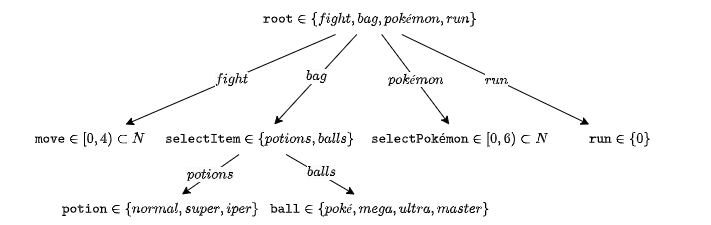
\includegraphics[width=\textwidth]{figs/decisions.drawio.png}
    \caption{Esempio di albero delle decisioni, usando come esempio il combattimento
    nel gioco dei Pokémon. Un esempio di decision path:\\
    \code{\{root: bag, select\_item: potions, potion: iper\}}}
    \label{fig:decisions}
\end{figure*}
\begin{figure*}
    \centering
    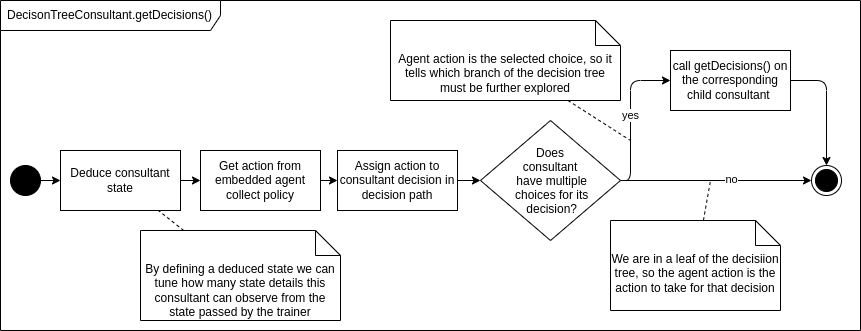
\includegraphics[width=\textwidth]{figs/decisions_getDecisions_activity_diagram.drawio.png}
    \caption{activity diagram per il metodo \code{getDecisions()} di un Consultant}
    \label{fig:decisions_getDecisions_activity_diagram}
\end{figure*}
\begin{figure*}
    \centering
    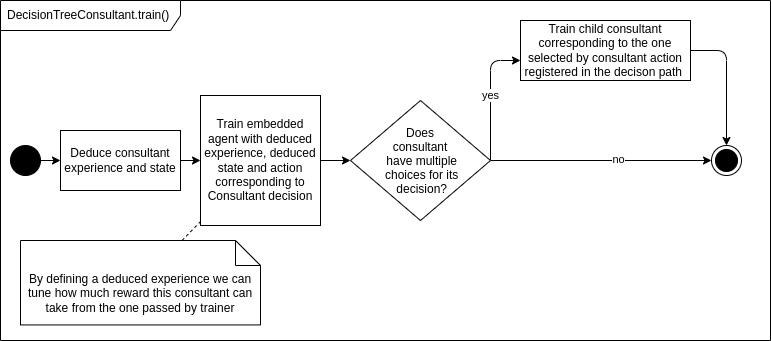
\includegraphics[width=\textwidth]{figs/decisions_train_activity_diagram.drawio.png}
    \caption{activity diagram per il metodo \code{train()} di un Consultant}
    \label{fig:decisions_train_activity_diagram}
\end{figure*}
\begin{figure*}
    \centering
    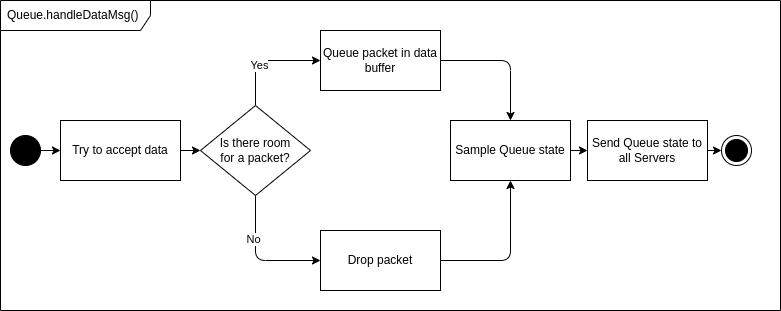
\includegraphics[width=\textwidth]{figs/queue_handleDataMsg_activity_diagram.drawio.png}
    \caption{activity diagram per la gestione dell'arrivo di un pacchetto nella coda}
    \label{fig:queue_handleDataMsg_activity_diagram}
\end{figure*}
\begin{figure*}
    \centering
    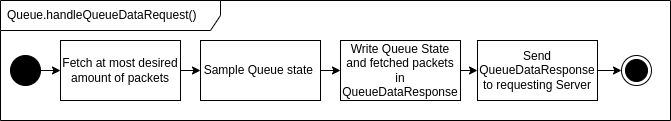
\includegraphics[width=\textwidth]{figs/queue_handleQueueDataRequest_activity_diagram.drawio.png}
    \caption{activity diagram per la gestione di una richiesta di dati da parte di un servente di pacchetti nella coda}
    \label{fig:queue_handleQueueDataRequest_activity_diagram}
\end{figure*}
\begin{figure*}
    \centering
    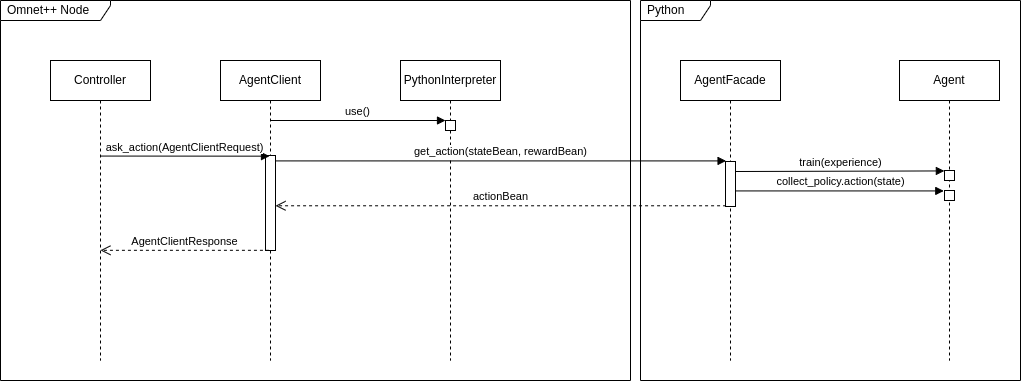
\includegraphics[width=\textwidth]{figs/agentc_sequence_diagram.drawio.png}
    \caption{sequence diagram per la servitura di una richiesta di azione del Controller nei confronti dell'agente.}
    \label{fig:agentc_sequence_diagram}
\end{figure*}
\begin{figure*}
    \centering
    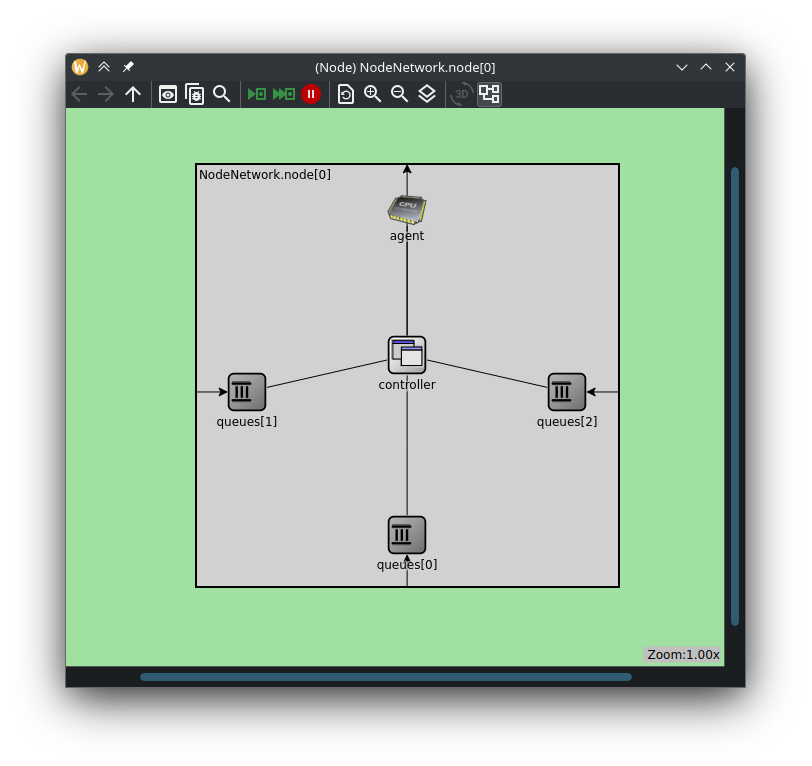
\includegraphics[width=\textwidth]{figs/node_layout_3queues.png}
    \caption{Nodo con tre code}
    \label{fig:node_layout_3queues}
\end{figure*}
\begin{figure*}
    \centering
    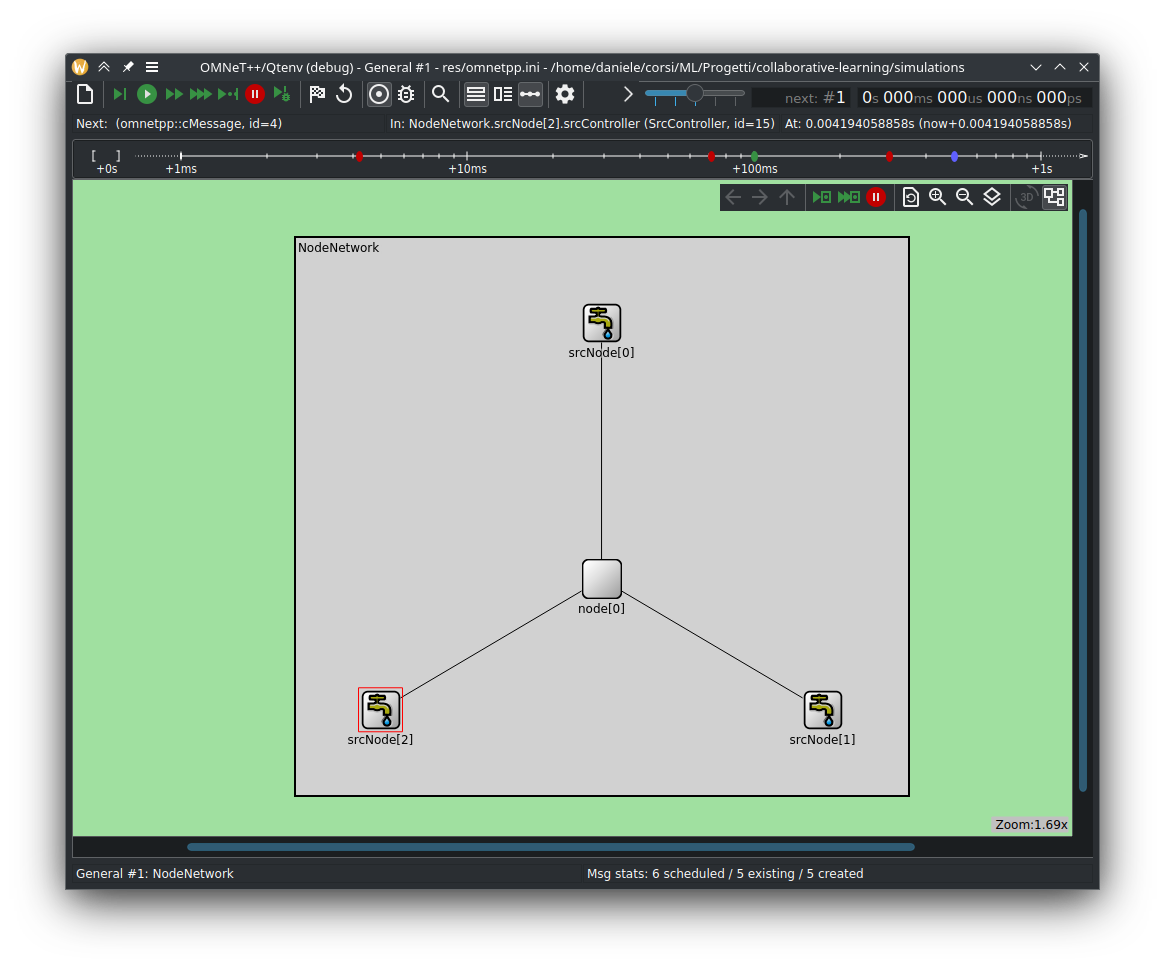
\includegraphics[width=\textwidth]{figs/network_layout_3queues.png}
    \caption{Rete con tre nodi sorgente e un solo nodo con agente.}
    \label{fig:network_layout_3queues}
\end{figure*}

\end{document}